\chapter{Вёрстка таблиц} \label{chapt3}

\section{Таблица обыкновенная} \label{sect3_1}

Так размещается таблица:

\begin{table} [htbp]
  \centering
  \changecaptionwidth\captionwidth{15cm}
  \caption{Название таблицы}\label{Ts0Sib}%
  \begin{tabular}{| p{3cm} || p{3cm} | p{3cm} | p{4cm}l |}
  \hline
  \hline
  Месяц   & \centering $T_{min}$, К & \centering $T_{max}$, К &\centering  $(T_{max} - T_{min})$, К & \\
  \hline
  Декабрь &\centering  253.575   &\centering  257.778    &\centering      4.203  &   \\
  Январь  &\centering  262.431   &\centering  263.214    &\centering      0.783  &   \\
  Февраль &\centering  261.184   &\centering  260.381    &\centering     $-$0.803  &   \\
  \hline
  \hline
  \end{tabular}
\end{table}

\begin{table} [htbp]% Пример записи таблицы с номером, но без отображаемого наименования
    \centering
    \parbox{9cm}{% чтобы лучше смотрелось, подбирается самостоятельно
        \captiondelim{}% должен стоять до самого пустого caption
        \caption{}%
        \label{tbl:test1}%
        \begin{SingleSpace}
            \begin{tabular}{| c | c | c | c |}
                \hline
                Оконная функция & ${2N}$& ${4N}$& ${8N}$\\ \hline
                Прямоугольное   & 8.72  & 8.77  & 8.77  \\ \hline
                Ханна           & 7.96  & 7.93  & 7.93  \\ \hline
                Хэмминга        & 8.72  & 8.77  & 8.77  \\ \hline
                Блэкмана        & 8.72  & 8.77  & 8.77  \\ \hline
            \end{tabular}%
        \end{SingleSpace}
    }
\end{table}

Таблица \ref{tbl:test2} "--- пример таблицы, оформленной в~классическом книжном
варианте или~очень близко к~нему. \mbox{ГОСТу} по~сути не~противоречит. Можно
ещё~улучшить представление, с~помощью пакета \verb|siunitx| или~подобного.

\begin{table} [htbp]%
    \centering
    \caption{Наименование таблицы, очень длинное наименование таблицы, чтобы посмотреть как оно будет располагаться на~нескольких строках и~переноситься}%
    \label{tbl:test2}% label всегда желательно идти после caption
    \renewcommand{\arraystretch}{1.5}%% Увеличение расстояния между рядами, для улучшения восприятия.
    \begin{SingleSpace}
        \begin{tabular}{@{}@{\extracolsep{20pt}}llll@{}} %Вертикальные полосы не используются принципиально, как и лишние горизонтальные (допускается по ГОСТ 2.105 пункт 4.4.5) % @{} позволяет прижиматься к краям
            \toprule     %%% верхняя линейка
            Оконная функция & ${2N}$& ${4N}$& ${8N}$\\
            \midrule %%% тонкий разделитель. Отделяет названия столбцов. Обязателен по ГОСТ 2.105 пункт 4.4.5 
            Прямоугольное   & 8.72  & 8.77  & 8.77  \\
            Ханна           & 7.96  & 7.93  & 7.93  \\
            Хэмминга        & 8.72  & 8.77  & 8.77  \\
            Блэкмана        & 8.72  & 8.77  & 8.77  \\
            \bottomrule %%% нижняя линейка
        \end{tabular}%
    \end{SingleSpace}
\end{table}

\section{Таблица с многострочными ячейками и примечанием}

Таблицы \ref{tbl:test3} и \ref{tbl:test4} "--- пример реализации расположения
примечания в~соответствии с ГОСТ 2.105. Каждый вариант со своими достоинствами
и~недостатками. Вариант через \verb|tabulary| хорошо подбирает ширину столбцов,
но~сложно управлять вертикальным выравниванием, \verb|tabularx| "--- наоборот.




\section{Параграф "--- два} \label{sect3_2}

Пример картинок с профилями цвета:

\begin{figure}[h]
  \centering
  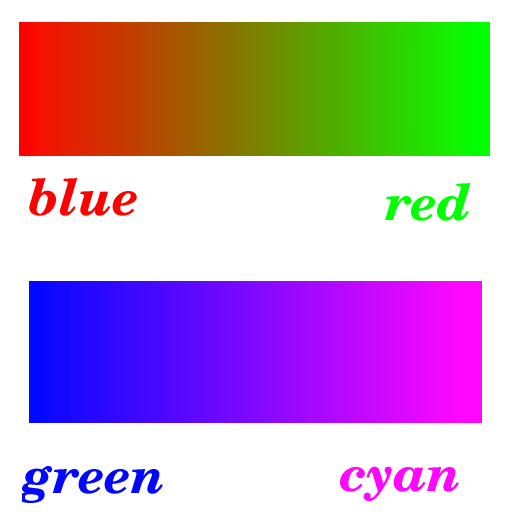
\includegraphics[width=5cm]{png-color-profile-test_orig.png}
  \caption{оригинальная картинка с профилем (не-ICCBased), взятая с \href{https://forums.adobe.com/thread/1183489}{форума Adobe}. Если наблюдаемые цвета не соответствуют надписям - значит с профилями что-то не так.
  У меня в texlive 2018 не работает ни в lualatex, ни в xelatex, ни в pdflatex.}
  \label{img:orig pic with profile}
\end{figure}

\begin{figure}[!htb]
	\noindent
	\begin{minipage}{0.5\textwidth}	
		\hfill
		
\includegraphics[height=14.1cm]{colorbar.png}%	
		\hspace{1cm}
	\end{minipage}%
	\hfill%
	\begin{minipage}{0.5\textwidth}
		\begin{tabular}{p{1.5cm} p{1cm} p{1.5cm} p{1cm}}
          \cellcolor[rgb]{1.00000,1.00000,1.00000}{~} & ~ & \cellcolor[cmyk]{0.00000,0.00060,0.00027,0.00014}{~} & {color1} \\
          \cellcolor[rgb]{0.50196,0.50196,0.50196}{~} & ~ & \cellcolor[cmyk]{0.24808,0.20929,0.19661,0.36100}{~} & {color2} \\
          \cellcolor[rgb]{0.00000,0.00000,0.00000}{~} & ~ & \cellcolor[cmyk]{0.00000,0.00000,0.00000,0.99997}{~} & {color3} \\
          \cellcolor[rgb]{1.00000,0.75294,0.75294}{~} & ~ & \cellcolor[cmyk]{0.00482,0.36851,0.22217,0.00104}{~} & {color4} \\
          \cellcolor[rgb]{0.00000,0.50196,0.50196}{~} & ~ & \cellcolor[cmyk]{0.83091,0.21785,0.40542,0.07037}{~} & {color5} \\
          \cellcolor[rgb]{0.00000,1.00000,1.00000}{~} & ~ & \cellcolor[cmyk]{0.84741,0.00000,0.02052,0.00026}{~} & {color6} \\
          \cellcolor[rgb]{0.00000,0.75294,0.00000}{~} & ~ & \cellcolor[cmyk]{0.78500,0.00000,0.99997,0.00032}{~} & {color7} \\
          \cellcolor[rgb]{0.00000,0.25098,0.00000}{~} & ~ & \cellcolor[cmyk]{0.74954,0.41801,0.83082,0.63682}{~} & {color8} \\
          \cellcolor[rgb]{0.50196,0.00000,0.00000}{~} & ~ & \cellcolor[cmyk]{0.26699,0.98015,0.81404,0.43252}{~} & {color9} \\
          \cellcolor[rgb]{0.75294,0.25098,0.00000}{~} & ~ & \cellcolor[cmyk]{0.08933,0.89926,0.96097,0.06418}{~} & {color10} \\
          \cellcolor[rgb]{0.00000,1.00000,0.00000}{~} & ~ & \cellcolor[cmyk]{0.64434,0.00000,0.99997,0.00000}{~} & {color11} \\
          \cellcolor[rgb]{1.00000,0.00000,0.00000}{~} & ~ & \cellcolor[cmyk]{0.00012,0.99997,0.99840,0.01167}{~} & {color12} \\
          \cellcolor[rgb]{1.00000,0.00000,0.60000}{~} & ~ & \cellcolor[cmyk]{0.00627,0.99583,0.05092,0.00235}{~} & {color13} \\
          \cellcolor[rgb]{1.00000,0.50196,0.00000}{~} & ~ & \cellcolor[cmyk]{0.00317,0.75140,0.98398,0.00516}{~} & {color14} \\
          \cellcolor[rgb]{0.50196,0.50196,1.00000}{~} & ~ & \cellcolor[cmyk]{0.80249,0.35647,0.00000,0.00034}{~} & {color15} \\
          \cellcolor[rgb]{0.47451,0.20000,0.82353}{~} & ~ & \cellcolor[cmyk]{0.77577,0.84265,0.00000,0.00157}{~} & {color16} \\
          \cellcolor[rgb]{1.00000,1.00000,0.00000}{~} & ~ & \cellcolor[cmyk]{0.05483,0.00124,0.97897,0.00024}{~} & {color17} \\
          \cellcolor[rgb]{1.00000,0.50196,0.50196}{~} & ~ & \cellcolor[cmyk]{0.00673,0.76382,0.56541,0.00029}{~} & {color18} \\
          \cellcolor[rgb]{0.20000,0.40000,0.00000}{~} & ~ & \cellcolor[cmyk]{0.74580,0.29775,0.94908,0.26606}{~} & {color19} \\
		\end{tabular}%
	\end{minipage}%
	\caption{Слева --- растровая картинка, png, RGB (xcolor не влияет) \newline
			 по центру --- столбец таблицы с заливкой заданной в RGB (xcolor влияет), 
			 справа --- столбец таблицы с заливкой заданной в CMYK (xcolor влияет)}
\end{figure}%

\newlength{\picw}
\setlength{\picw}{3cm}
\clearpage
\begin{longtable}[c]{|b{\picw}|b{\picw}|b{8cm}|}
    \hline     %%% верхняя линейка
    png & jpg & пояснение \\            
    \midrule
    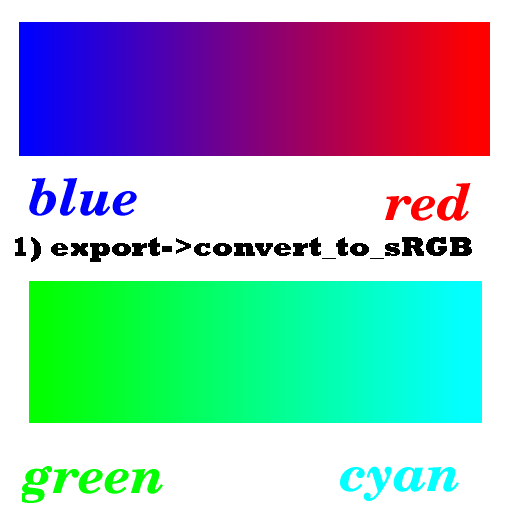
\includegraphics[width=\picw]{1_export_convert_to_sRGB.png} & 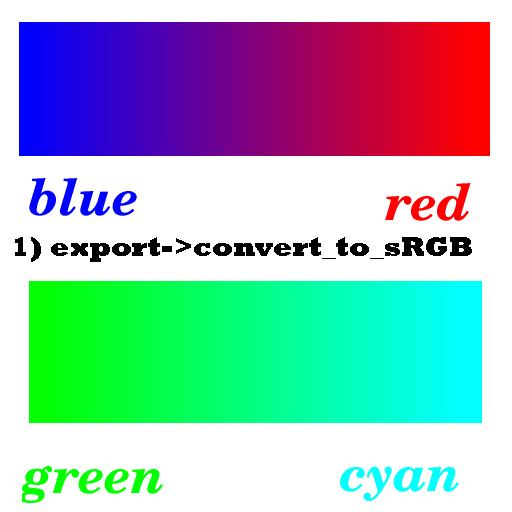
\includegraphics[width=\picw]{1_export_convert_to_sRGB.jpg} & 
    профиль \enquote{применился}, и сохранено без профиля. В любом случае отображается правильно. \\  
    \midrule
    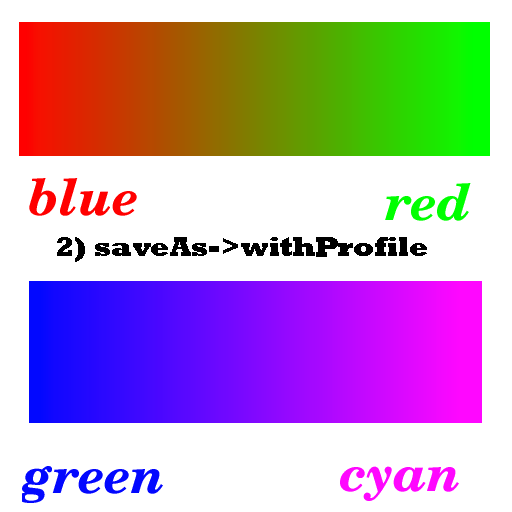
\includegraphics[width=\picw]{2_saveAs_with_profile.png} & 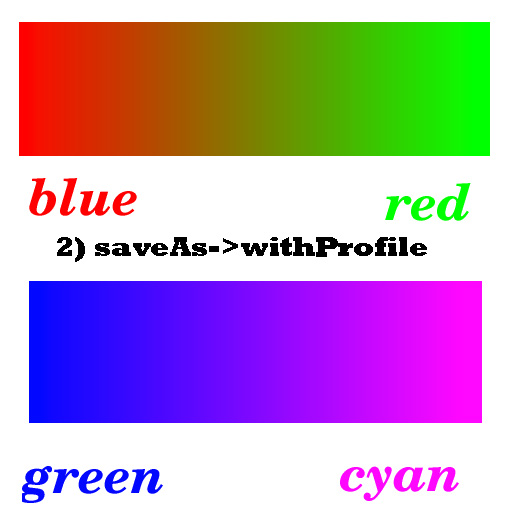
\includegraphics[width=\picw]{2_saveAs_with_profile.jpg} & 
    аналогично исходному изображению, цвета картинки записаны как BRG, а профиль это \enquote{исправляет}.
    \\  \midrule
    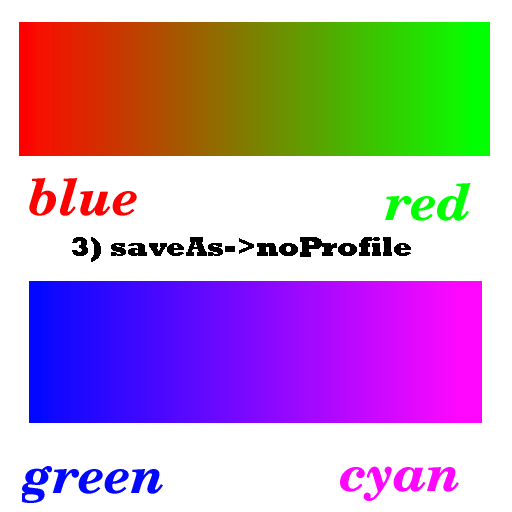
\includegraphics[width=\picw]{3_saveAs_noProfile.png} & 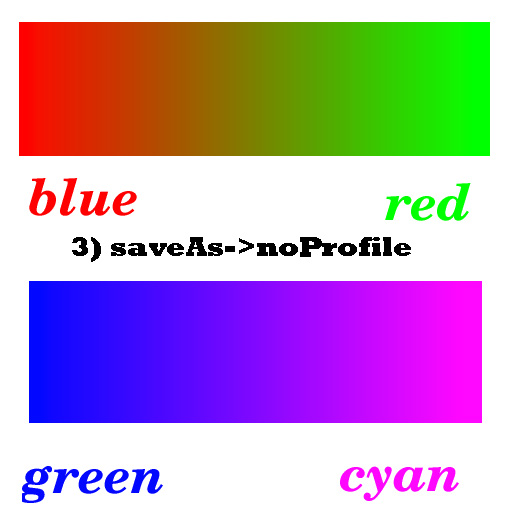
\includegraphics[width=\picw]{3_saveAs_noProfile.jpg} & 
    исходное изображение сохранено с \enquote{отбрасываением} профиля. Если предыдущая строчка выглядит как эта --- значит там тоже профиль отброшен.
    \\  \midrule
    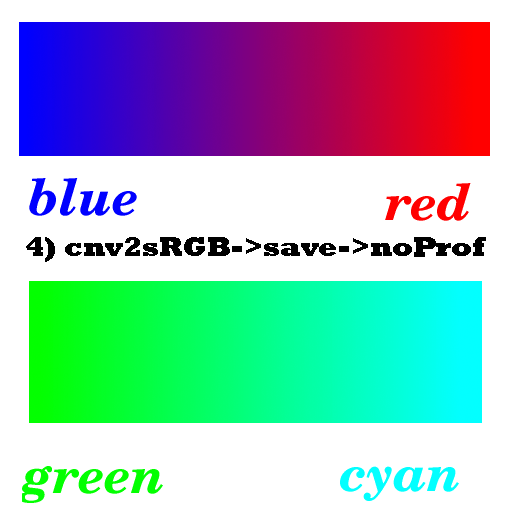
\includegraphics[width=\picw]{4_cnv2sRGB_saveAs_noProfile.png} & 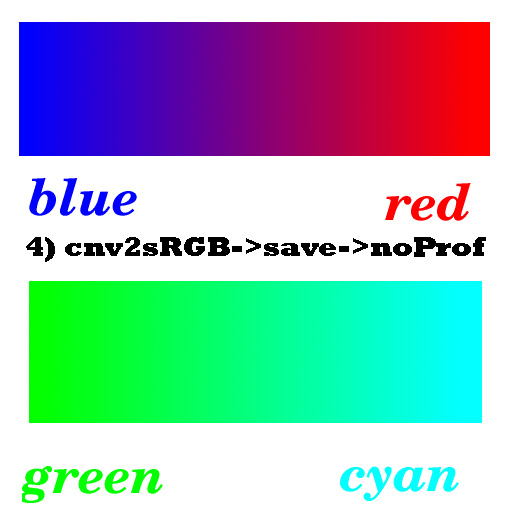
\includegraphics[width=\picw]{4_cnv2sRGB_saveAs_noProfile.jpg} & 
    явно выполнено пробразование в sRGB, сохранено без профиля.
    \\  \midrule
    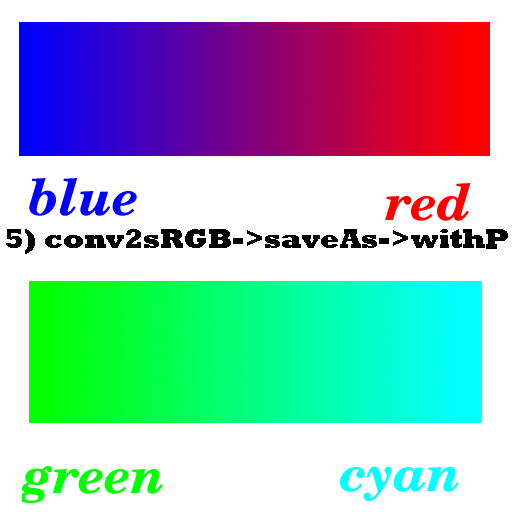
\includegraphics[width=\picw]{5_cnv2sRGB_saveAs_withProfile.png} & 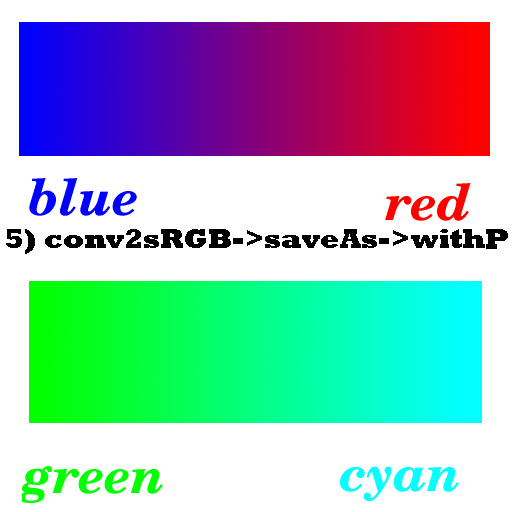
\includegraphics[width=\picw]{5_cnv2sRGB_saveAs_withProfile.jpg} & 
    явно выполнено пробразование в sRGB, сохранено с профилем (который ничего не меняет).
    \\  \midrule
    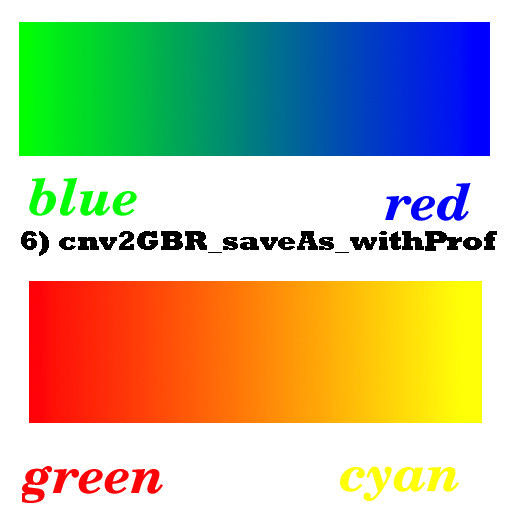
\includegraphics[width=\picw]{6_cnv2GBR_saveAs_withProfile.png} & 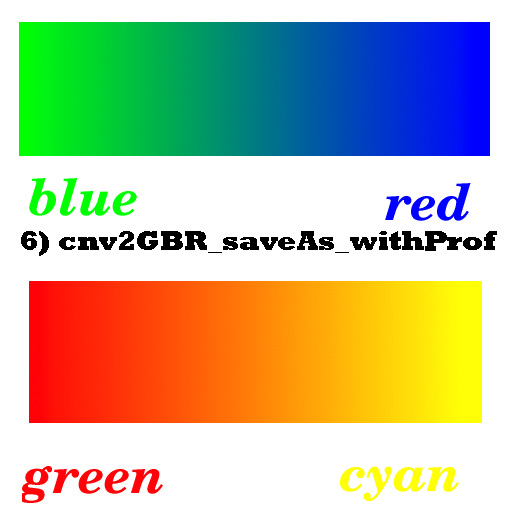
\includegraphics[width=\picw]{6_cnv2GBR_saveAs_withProfile.jpg} & 
    icc-based colorspace, где primaries как \enquote{ITU-R BT.709}, но переставлены местами как GBR, 
    а профиль это исправляет, сохранено с профилем.
    \\ \midrule
    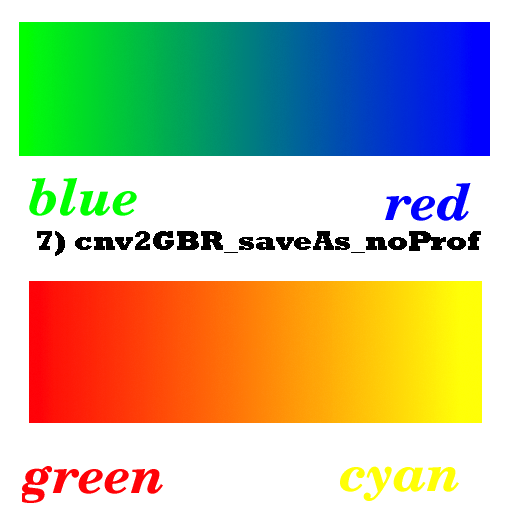
\includegraphics[width=\picw]{7_cnv2GBR_saveAs_noProfile.png} & 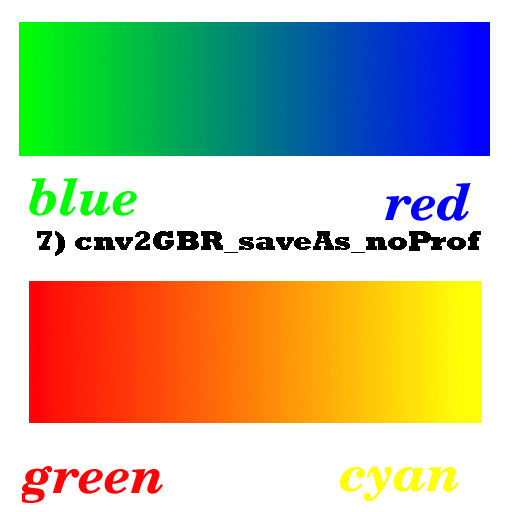
\includegraphics[width=\picw]{7_cnv2GBR_saveAs_noProfile.jpg} & 
    то же, но сохранено с отбрасыванием профиля
    \\
    \bottomrule %%% нижняя линейка
\end{longtable}%    


\section{Параграф с подпараграфами} \label{sect3_3}

\subsection{Подпараграф "--- один} \label{subsect3_3_1}

Некоторый текст.

\subsection{Подпараграф "--- два} \label{subsect3_3_2}

Некоторый текст.

\clearpage